\chapter{Recursive Jigsaw Reconstruction for Events with Missing Energy and Identifying ISR Jets}
\label{chap:jigsaw}

\section{Introduction to Recursive Jigsaw Algorithm on Events with \MET}
\label{Jigsaw:Intro}

\indent Every search involving missing energy has to contend with the fact that information on the invisible system is lost.  The question of how to best fill the missing degree of freedom is a problem ubiquitous to all analysis that have \MET especially when there exists multiple invisible particles in the event. The recursive jigsaw method aims to compartmentalize the lost information and gain the most from what information that is available.\\
\indent Traditional edge variables such as $M_{T2}$, shown in equation \ref{eqnMT2}, extremize over all possible kinematic configurations of the two invisible particles ${\bf p}_1$ and ${\bf p}_2$ to find some sort of kinematic edge.  In effect, $M_{T2}$ is an extremization over all possible configurations allowed by the ambiguity due to not being able to directly measure all aspects of the two invisible particles.  However, over optimizing over a large phase space to pin down the unknown degrees of freedom can unintentionally destroy useful information.  \\
\begin{equation}
\label{eqnMT2}
M^{2}_{T2} \equiv \mymin[\slashed{\bf p}_{1}+\slashed{\bf p}_{2}=\slashed{\bf E}_{T}^{miss}]  \Big[ \mymax[] \{ m_{T}^{2}({\bf p}_{Tl-},\slashed{\bf p}_{1}), m_{T}^{2}({\bf p}_{Tl+},\slashed{\bf p}_{2})\} \Big]
\end{equation}
\indent The recursive jigsaw reconstruction (RJR) method also uses maximizations and minimizations to pin down the degrees of freedom left open by lost information.  However, these extremizations are restricted to the specific location of the visible particle in its decay tree.  Imagine a simple particle decay chain where $a \rightarrow b~c$ and then $c \rightarrow 1~2$.  Recursive jigsaw would treat the situation differently if particle $1$ was invisible compared to if particle $b$ was invisible.  To zeroth order, losing information about particle $1$ affects only half the information on particle $c$ which contains only half the information of particle $a$, but losing information on particle $b$ directly affects half the information on particle $a$.   Unlike traditional methods which extremizes over all possible configurations of the invisible particle. RJR compartmentalizes the lost information and extracts the maximum amount of information from events with missing energy.  \\
\indent RJR separates the event according to a predefined "decay tree."  For compressed region, the most basic tree involve separating the event into sparticle and ISR systems and then further separating the sparticle system into visible and invisible parts. The decay tree is represented in figure.~\ref{fig:DecayTree}.
\begin{figure}[h]
\centering
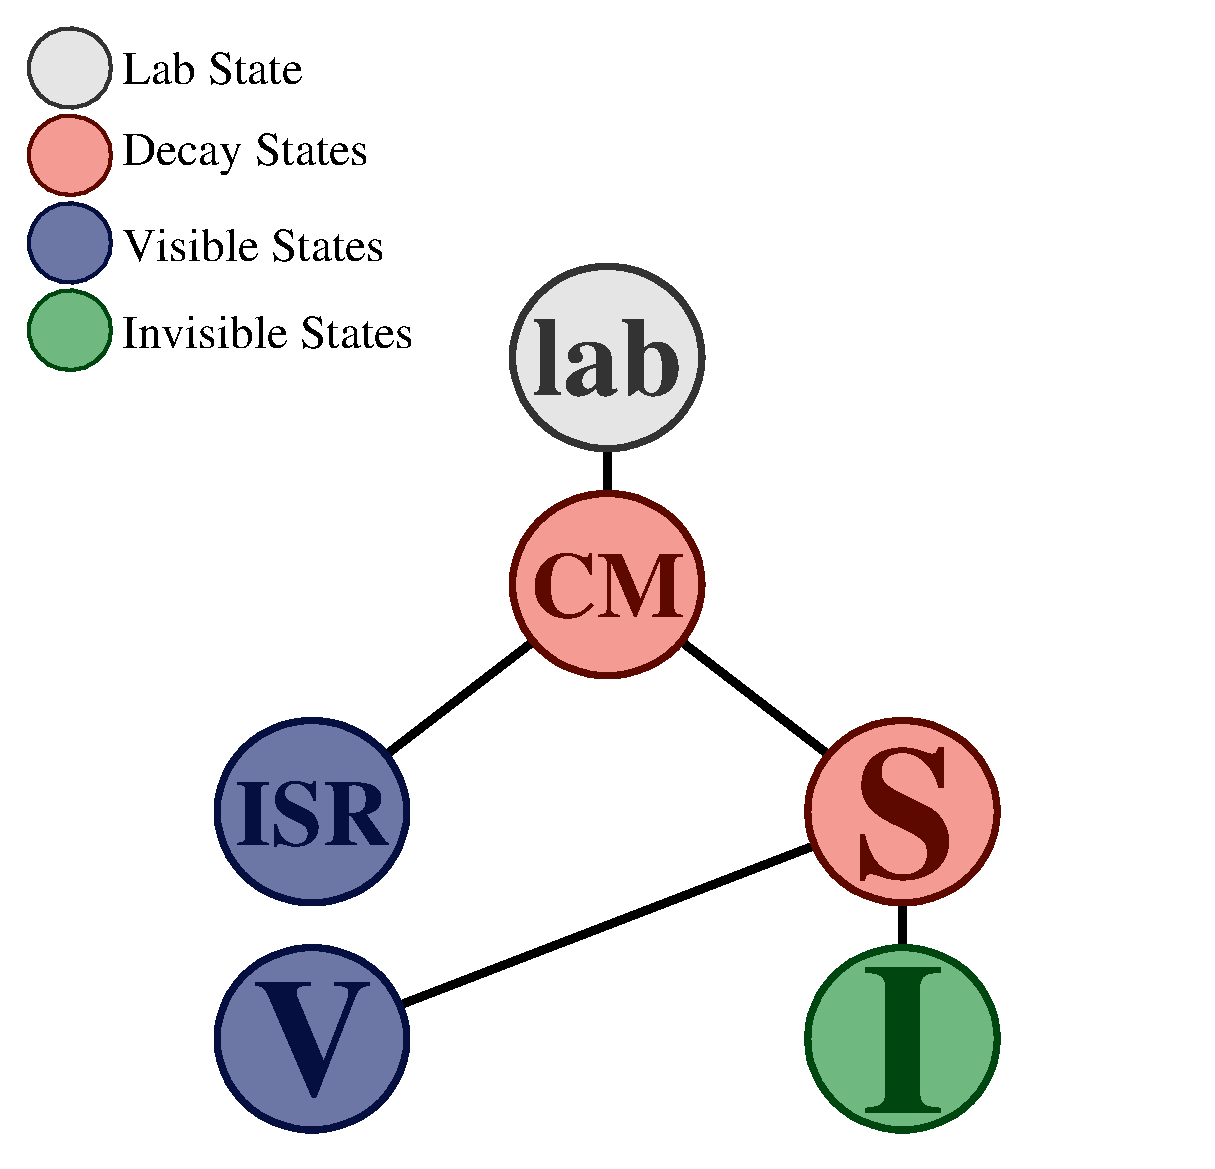
\includegraphics[width=0.6\textwidth]{./figures/DecayTree.eps}
\caption{Decay Tree corresponding to ISR-assisted \MET signal analysis strategy. \label{fig:DecayTree}}
\end{figure}\\

Each node in the decay tree represent a particular intermediate state or final state.  RJR will classify all accepted objects into the different nodes according to a specific set of rules detailed in section \ref{Jigsaw:ISR}.  The rules overcomes combinatoric ambiguities and sets the unknown degree of freedoms associated with all weakly interacting final state particles according to maximizations and minimizations.   \\
The decay tree can be as detailed as needed be, either attempting to resolve every branch in the decay tree down to the level of the final state objects or forming generic aggregate intermediate states that have useful kinematics.   

\section{Recursive Jigsaw Method of Identifying Initial State Radiation}
\label{Jigsaw:ISR}

In order to separate the event into an initial state radiation (ISR) system and a sparticle system, we first boost to the transverse center of mass frame of all accepted objects.  This transverse center of mass frame has symmetries that we would like to exploit.  The most important property of the transverse center of mass frame is that if the entire event is divided into two systems, these two systems must have equal and opposite transverse momenta.  The other important point to note is that the lab frame and the transverse center of mass frame significantly differ only in cases when an energetic object is not accepted.  In other words, the two frames differ significantly only when the \MET has a high probability of being miss reconstructed. \\

Once in the transverse center of mass frame, we find the thrust axis $\vec{n}$ as defined in \ref{eqn:thrust}.  
\begin{equation}
\label{eqn:thrust}
\vec{n} \equiv \mymax{\vec{n}} \sum_i^{jets,~E^{miss}_T} |p_T^i \cdot \vec{n}|
\end{equation}
The thrust axis $\vec{n}$ represents the axis that maximizes the amount of transverse momenta along it.  The back to back recoil between ISR and stops should represent the single largest back to back kick in events with strong ISR.  As such, the thrust axis should approximate the direction of the back to back recoil between the stops and ISR.  We divide the event into two hemispheres according to the thrust axis.  The hemisphere containing the \MET is identified as the sparticle hemisphere containing the decay products of the two stops.  This is because we expect the sparticle hemisphere to contain the two \ninoone.  The hemisphere opposite the direction of the \MET is identified as the ISR hemisphere.  All jets in the ISR hemisphere are considered to have originated from initial state radiation and all jets in the sparticle hemisphere are considered to have originated from one of the two stops. \\
The thrust axis is ensured to maximize the amount of back to back $p_T$ because the total $p_T$ of the event is zero in the transverse center of mass frame. \\
There is a mathematically equivalent second interpretation of this method of ISR identification.  Since we are in the transverse center of mass frame, finding the thrust axis is the same as simultaneous maximizing the $p_T$ of the sparticle and ISR systems.  Since the total $E_T$ of the event is a constant, then maximizing the $p_T$ of the sparticle and ISR systems is identical to minimizing the masses of the sparticle and ISR systems.

\begin{equation}
\label{eqn:thrust}
E_T = \sqrt{(m^{ISR})^2+(p^{ISR}_{T})^2} + \sqrt{(m^{sparticle})^2+(p^{sparticle}_{T})^2}
\end{equation}

In this view, the ISR identification algorithm is an exclusive two jet clustering algorithm that seeks to simultaneously minimize the masses of both jets.  Again the two jets are guaranteed to have back to back jet axis because we in the transverse center of mass frame. 



\section{Performance of Initial State Radiation Identification Algorithm}
\label{Jigsaw:Performance}

We can check the performance of the thrust based initial state radiation (ISR) identification algorithm described in section \ref{Jigsaw:ISR} by plotting the ratio of reconstructed vs true ISR $p_T$ in signal simulation.  Figure \ref{fig:ISRPerformance} shows the distribution of the ratio of reconstructed vs true ISR $p_T$ for $350$ GeV stop mass and $172$ GeV neutralino mass signal sample.  Only events with fully hadronic stop decays and at least $400$ GeV of true ISR $p_T$ are accepted for this plot.  Detector resolution effects on jets and \met are included when calculating the reconstructed ISR $p_T$.

\begin{figure}[h]
\centering
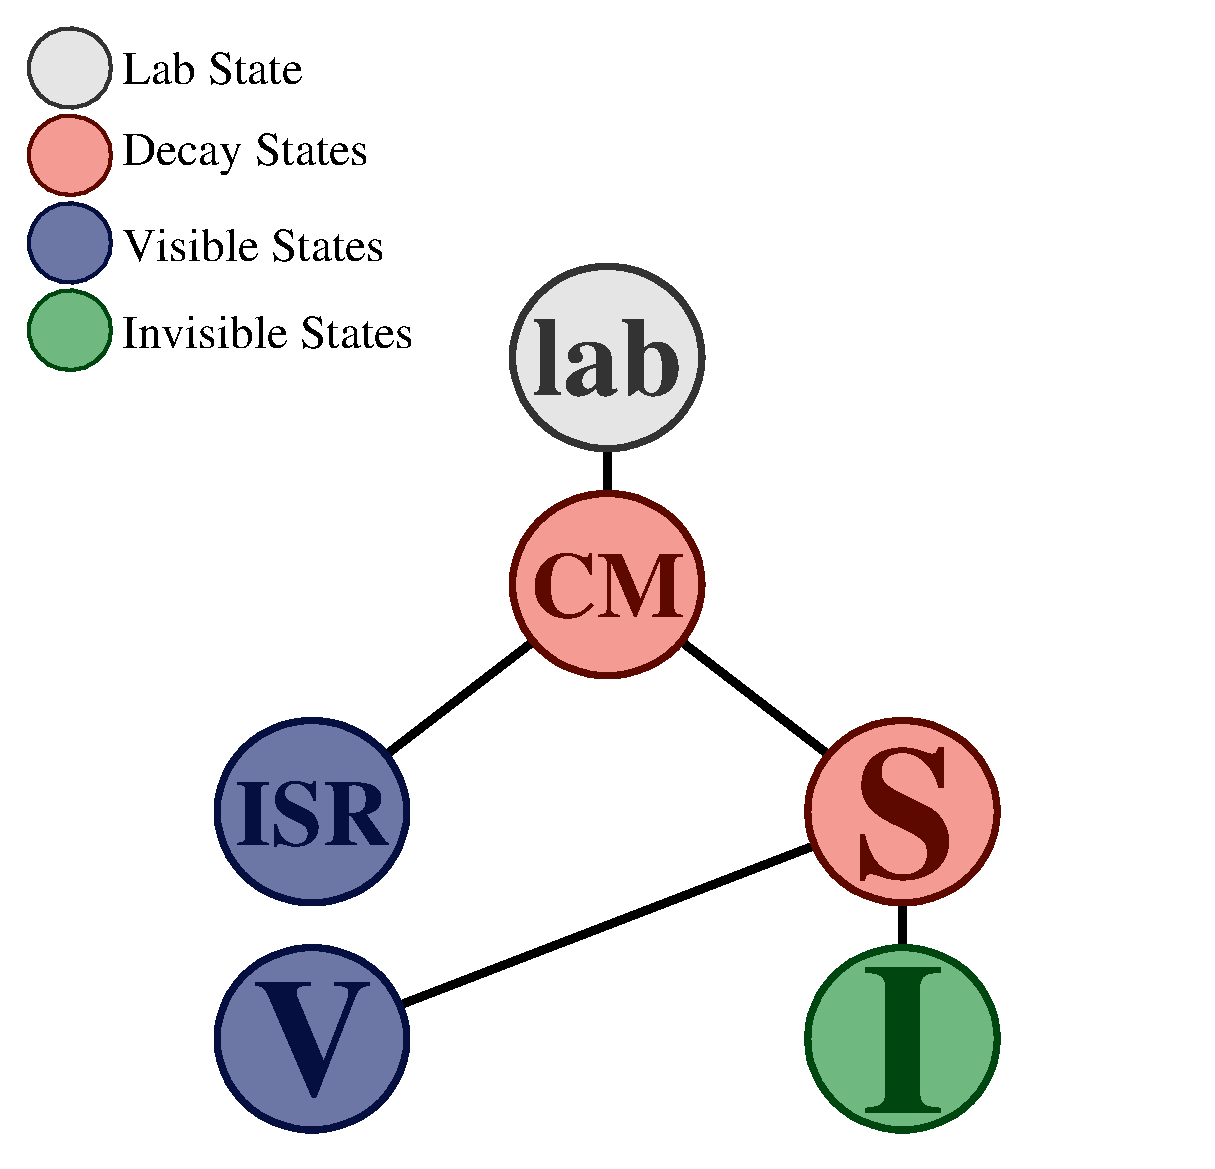
\includegraphics[width=0.6\textwidth]{./figures/DecayTree.eps}
\caption{The distribution of the ratio of reconstructed vs true ISR $p_T$ for the $350$ GeV stop mass and $172$ GeV neutralino mass signal sample.  Only simulations with fully hadronic stop decays and at least $400$ GeV of true ISR $p_T$ are accepted.  The red distribution is formed when the whole ISR system is equated to just the highest $p_T$ jet.  The blue distribution uses the thrust based ISR identification system.  \label{fig:ISRPerformance}}
\end{figure}

A simple and currently popular form of ISR identification is simply the equating the highest $p_T$ jet with the ISR system. This algorithm is represented by the distribution in red in figure \ref{fig:ISRPerformance}.  We see that the simple highest $p_T$ jet algorithm often fails to capture the full $p_T$ of the ISR system because the ISR system's energy is split between multiple jets.  $20$ to $50$ percent of the ISR energy is not reconstructed about $40$ percent of the time when we use the highest $p_T$ jet ISR identification algorithm.\\

In contrast the thrust based ISR identification system is able to capture the total $p_T$ of the ISR system quiet well.  The fitted gaussian width of the blue peak is only $9$ percent and this includes detector resolution effects.  The gaussian mean is not centered about zero but instead is centered about $1.05$.  The reason for this is because a jet originating from a stop will occasionally go in the opposite direction as the \met and be misidentified as an ISR jet.  The $p_T$ of the misidentified sparticle jet tend to be small relativity to the $p_T$ of the ISR system as a whole.  Therefore this misidentification shows up as a $5$ percent bias in the reconstructed ISR $p_T$.  Optimization of the ISR identification algorithm shows that this small bias does not impact the sensitivity of the search.  \\

The non-gaussian tail in the blue distribution that exponentially decays to a reco vs true $p_T$ ratio of $1.5$ is due to energetic ISR jets that go in the same direction as the \MET.  In these cases, the ISR jets that are in the same direction as the \met are miss-reconstructed as having originated from a stop.  Only the ISR jets going in an opposite direction to the \MET are reconstructed as ISR jets.  The reconstructed ISR system fail to partially cancel the $p_T$ of the oppositely facing jets and the reconstructed ISR system has a larger $p_T$ then the true ISR $p_T$.  However, this case is rare and the non-gaussian tail accounts for less than $15$ percent of the events in blue distribution.

\section{Kinematic Variables of Initial State Radiation and Sparticle Systems}
\label{Jigsaw:Variables}

Once we separated the event into two hemispheres according the thrust axis as described in section \ref{Jigsaw:ISR} we can construct several variables that captures the kinematic properties of the two hemispheres.  The important variables are listed below.

\begin{description}
\item [\boldmath \NbV:] number of b-tagged jets associated with the sparticle hemisphere.
\item [\boldmath \NjV:] number of jets associated with the sparticle hemisphere.
\item [\boldmath \pTSBZero:] \pt\ of the leading b-tagged jet in the sparticle hemisphere.
\item [\boldmath \pTjV:] \pt\ of the fourth highest \pt\ jet in the sparticle hemisphere.
\item [\boldmath \MS:] transverse mass of the whole sparticle system and \met.
\item [\boldmath \PTISR:] \pt\ of the ISR system
\item [\boldmath \dphiISRI:] angular separation in $\phi$ of the ISR and the \met (evaluated in the transverse CM frame)
\item [\boldmath \RISR:] Ratio between \met and \PTISR (evaluated in transverse CM frame)
\end{description}

\NjV and \NbV quantify the jet multiplicity in the sparticle system.  \pTSBZero, \pTjV, \MS and \PTISR quantify the amount of energy in the sparticle and ISR hemispheres.  Finally, \dphiISRI and \RISR quantify the correlation between the ISR system and the \MET in direction and magnitude.  All of these variables will be used to separate signal from background in the signal region described in detail in section \ref{chap:SR}.

